\documentclass{../beamer_template/myBeamer}


\DeclareMathOperator{\Cov}{Cov}
\DeclareMathOperator{\Var}{Var}
\DeclareMathOperator{\E}{\mathbb{E}}
\DeclareMathOperator{\Proba}{\mathbb{P}}

\newcommand{\Covb}[2]{\ensuremath{\Cov\!\left[#1,#2\right]}}
\newcommand{\Eb}[1]{\ensuremath{\E\!\left[#1\right]}}
\newcommand{\Pb}[1]{\ensuremath{\Proba\!\left[#1\right]}}
\newcommand{\Varb}[1]{\ensuremath{\Var\!\left[#1\right]}}

% norm
%\newcommand{\norm}[1]{\| #1 \|}

\newcommand{\indep}{\rotatebox[origin=c]{90}{$\models$}}





\usepackage{mathptmx,amsmath,amssymb,graphicx,bibentry,bbm,babel,ragged2e}

\makeatletter


\renewcommand{\addlogo}{
	\hfill	
	
\includegraphics[height=.4cm]{../beamer_template/figures/logos/iconOM.png}
	
\includegraphics[scale=1]{../beamer_template/figures/logos/openmole_dark.png}
}


\newcommand{\noun}[1]{\textsc{#1}}
\newcommand{\jitem}[1]{\item \begin{justify} #1 \end{justify} \vfill{}}
%\newcommand{\sframe}[2]{\frame{\frametitle{#1}\addlogo #2}}

\newenvironment{centercolumns}{\begin{columns}[c]}{\end{columns}}
%\newenvironment{jitem}{\begin{justify}\begin{itemize}}{\end{itemize}\end{justify}}

%\usetheme{Warsaw}
%\setbeamertemplate{footline}[text line]{}
%\setbeamersize{text margin left=15pt,text margin right=15pt}
%\setbeamertemplate{headline}{}
%\setbeamertemplate{footline}[frame number]
%\setbeamertemplate{navigation symbols}{}

\usetheme{Darmstadt}
\setbeamertemplate{headline}{}
\setbeamertemplate{navigation symbols}{}
\setbeamercolor{palette quaternary}{fg=primaryDarkOM, bg=primaryGreenOM}


%\setbeamercovered{transparent}
%\setbeamercolor{structure}{fg=purple!50!blue, bg=purple!50!blue}

\@ifundefined{showcaptionsetup}{}{%
 \PassOptionsToPackage{caption=false}{subfig}}
\usepackage{subfig}

\usepackage[utf8]{inputenc}
%\usepackage[T1]{fontenc}


\usepackage{tikz}

\usepackage{multirow}

\usepackage{mdframed}

%\usepackage[usenames,dvipsnames]{pstricks}
%\usepackage{auto-pst-pdf}


%\usepackage[dvipsnames]{xcolor}

\usepackage{threeparttable}


\usepackage{listings}
\lstset{language=Java} 

\makeatother



\title[Case study model]{Case study: an epidemiological model}
%\subtitle{}
%\author[]{Yu Si-te$^1$}
\author{eX Modelo Summer School}
\date{August 31st, 2020}
%\institute{$^1$College of Public Health, Chongqing University\\
%
\includegraphics[width=0.3\textwidth]{figures/chongqing_medicaluniv}}

\begin{document}



\begin{frame}[plain]
	\titlepage
\end{frame}
\addtocounter{framenumber}{-1}

\AtBeginSection[]
{
	\frame{
		\tableofcontents[currentsection, hideallsubsections]
	}
	\addtocounter{framenumber}{-1}
}


% no need for outline
%\sframe{Outline}{
%\tableofcontents
%}

%Introducing a model 

%general purpose : spatial epidemio model

%scenarization

% - pedestrian dynamics



%
%X Pourquoi le logo OpenMOLE ??
%
%X Iceland (pas Island)
%XLudicrous
%X observational data
%
%Préciser que c’est un ABM et qu’est ce qu’un ABM.
%
%Est-ce que ça ne serait pas encore plus drôle si tu te présentais comme un Zombie Scientist ?
%
%Ne vaudrait-il pas mieux présenter direct le stade quarantine ?
%
%objective of the model number 1: better understanding the zombie attack process
%
%What is a potential model ?
%
%Lancer un coup la simu pour montrer qu’ils marchent / cours / vont vers les rescue zones, etc. Et donner l’url de la simu graphique
%
%presentation du sous modele : equipe qui bosse sur les mecanisems - les moins connu
%
%dire que gros modele - mais que params de coop les moins connus -> ce qu’on etudie
%
%montrer la GUI de coopeartion: https://om.exmodelo.org/coop/
%
%blouses + lunettes ?
%
%X logo du Mole institute
%
%X point de vue du scientifique qui vient, content que le modele soit etudie
%
%X model as black box, pas besoin de connaitre exacetement tous les processus et parameteres
%


\sframe{Decision making in a chaotic world}{

 % contextualize Center for Zombie Research
 % knowledge forgotten about how to use simulation models ? -> you are the last hope of the world
 %  point de vue du scientifique qui vient, content que le modele soit etudie

\centering

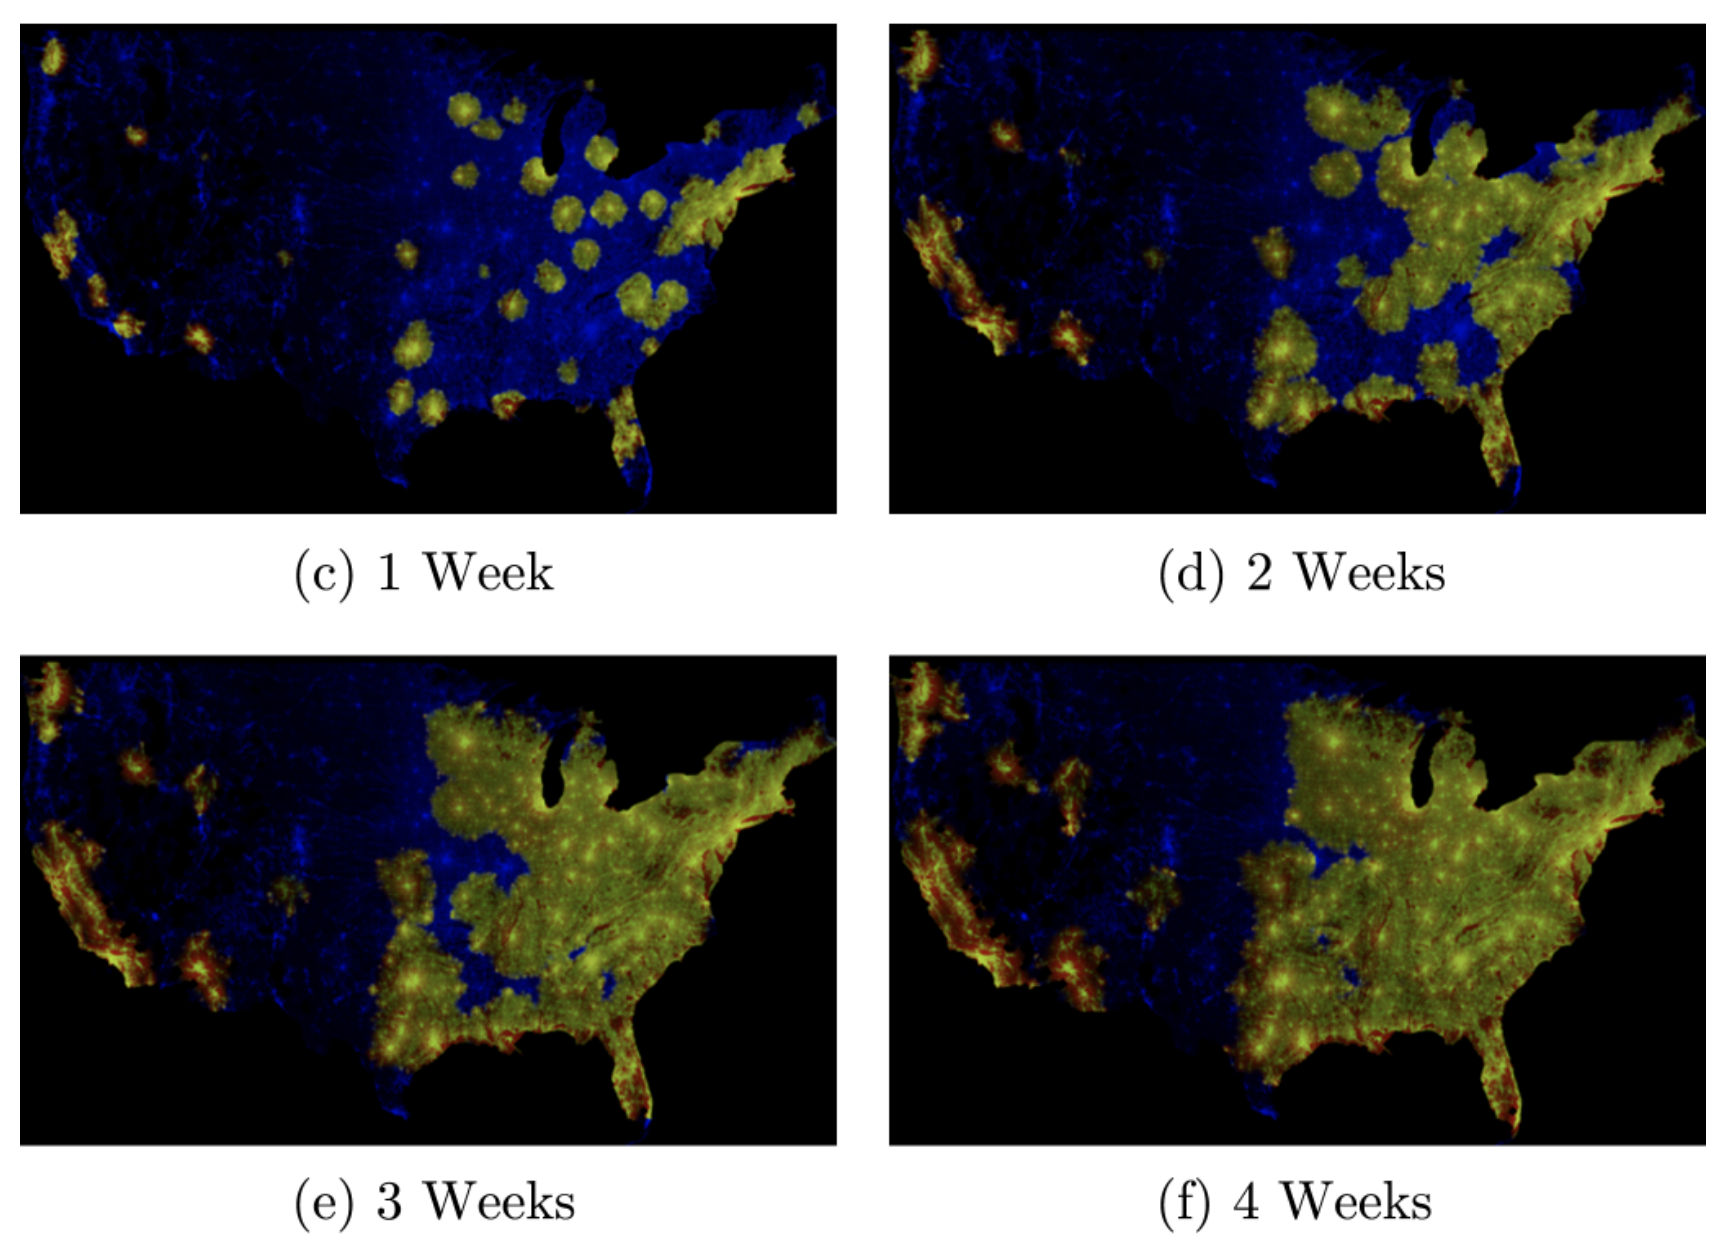
\includegraphics[width=\linewidth,height=0.8\textheight]{figures/zombieOutbreak.png}

\justify

\textit{Simulation of the 2010 Zombie outbreak in the US} \cite{alemi2015you}

}


\sframe{History of Zombie epidemiology}{

\begin{itemize}
	\item 2007: first outbreak in Iceland, relatively contained through ad-hoc measures
	\item 2010: it becomes pandemic
	\item 2010-2015: no clear records of events
	\item 2015-2018: reorganization of institutions, the MOLE (Medical Overview of Ludicrous Experiments) center in Chongqing gathers observational data from many local invasions across the world
	\item 2019: they released the first version of the model ZOMBIE (Zone of Optimal Management for Bacillus Infecting Everyone) and successfully applied
\end{itemize}

% 


}


\sframe{An operational model for local Zombie invasion}{

\justify



\begin{center}
%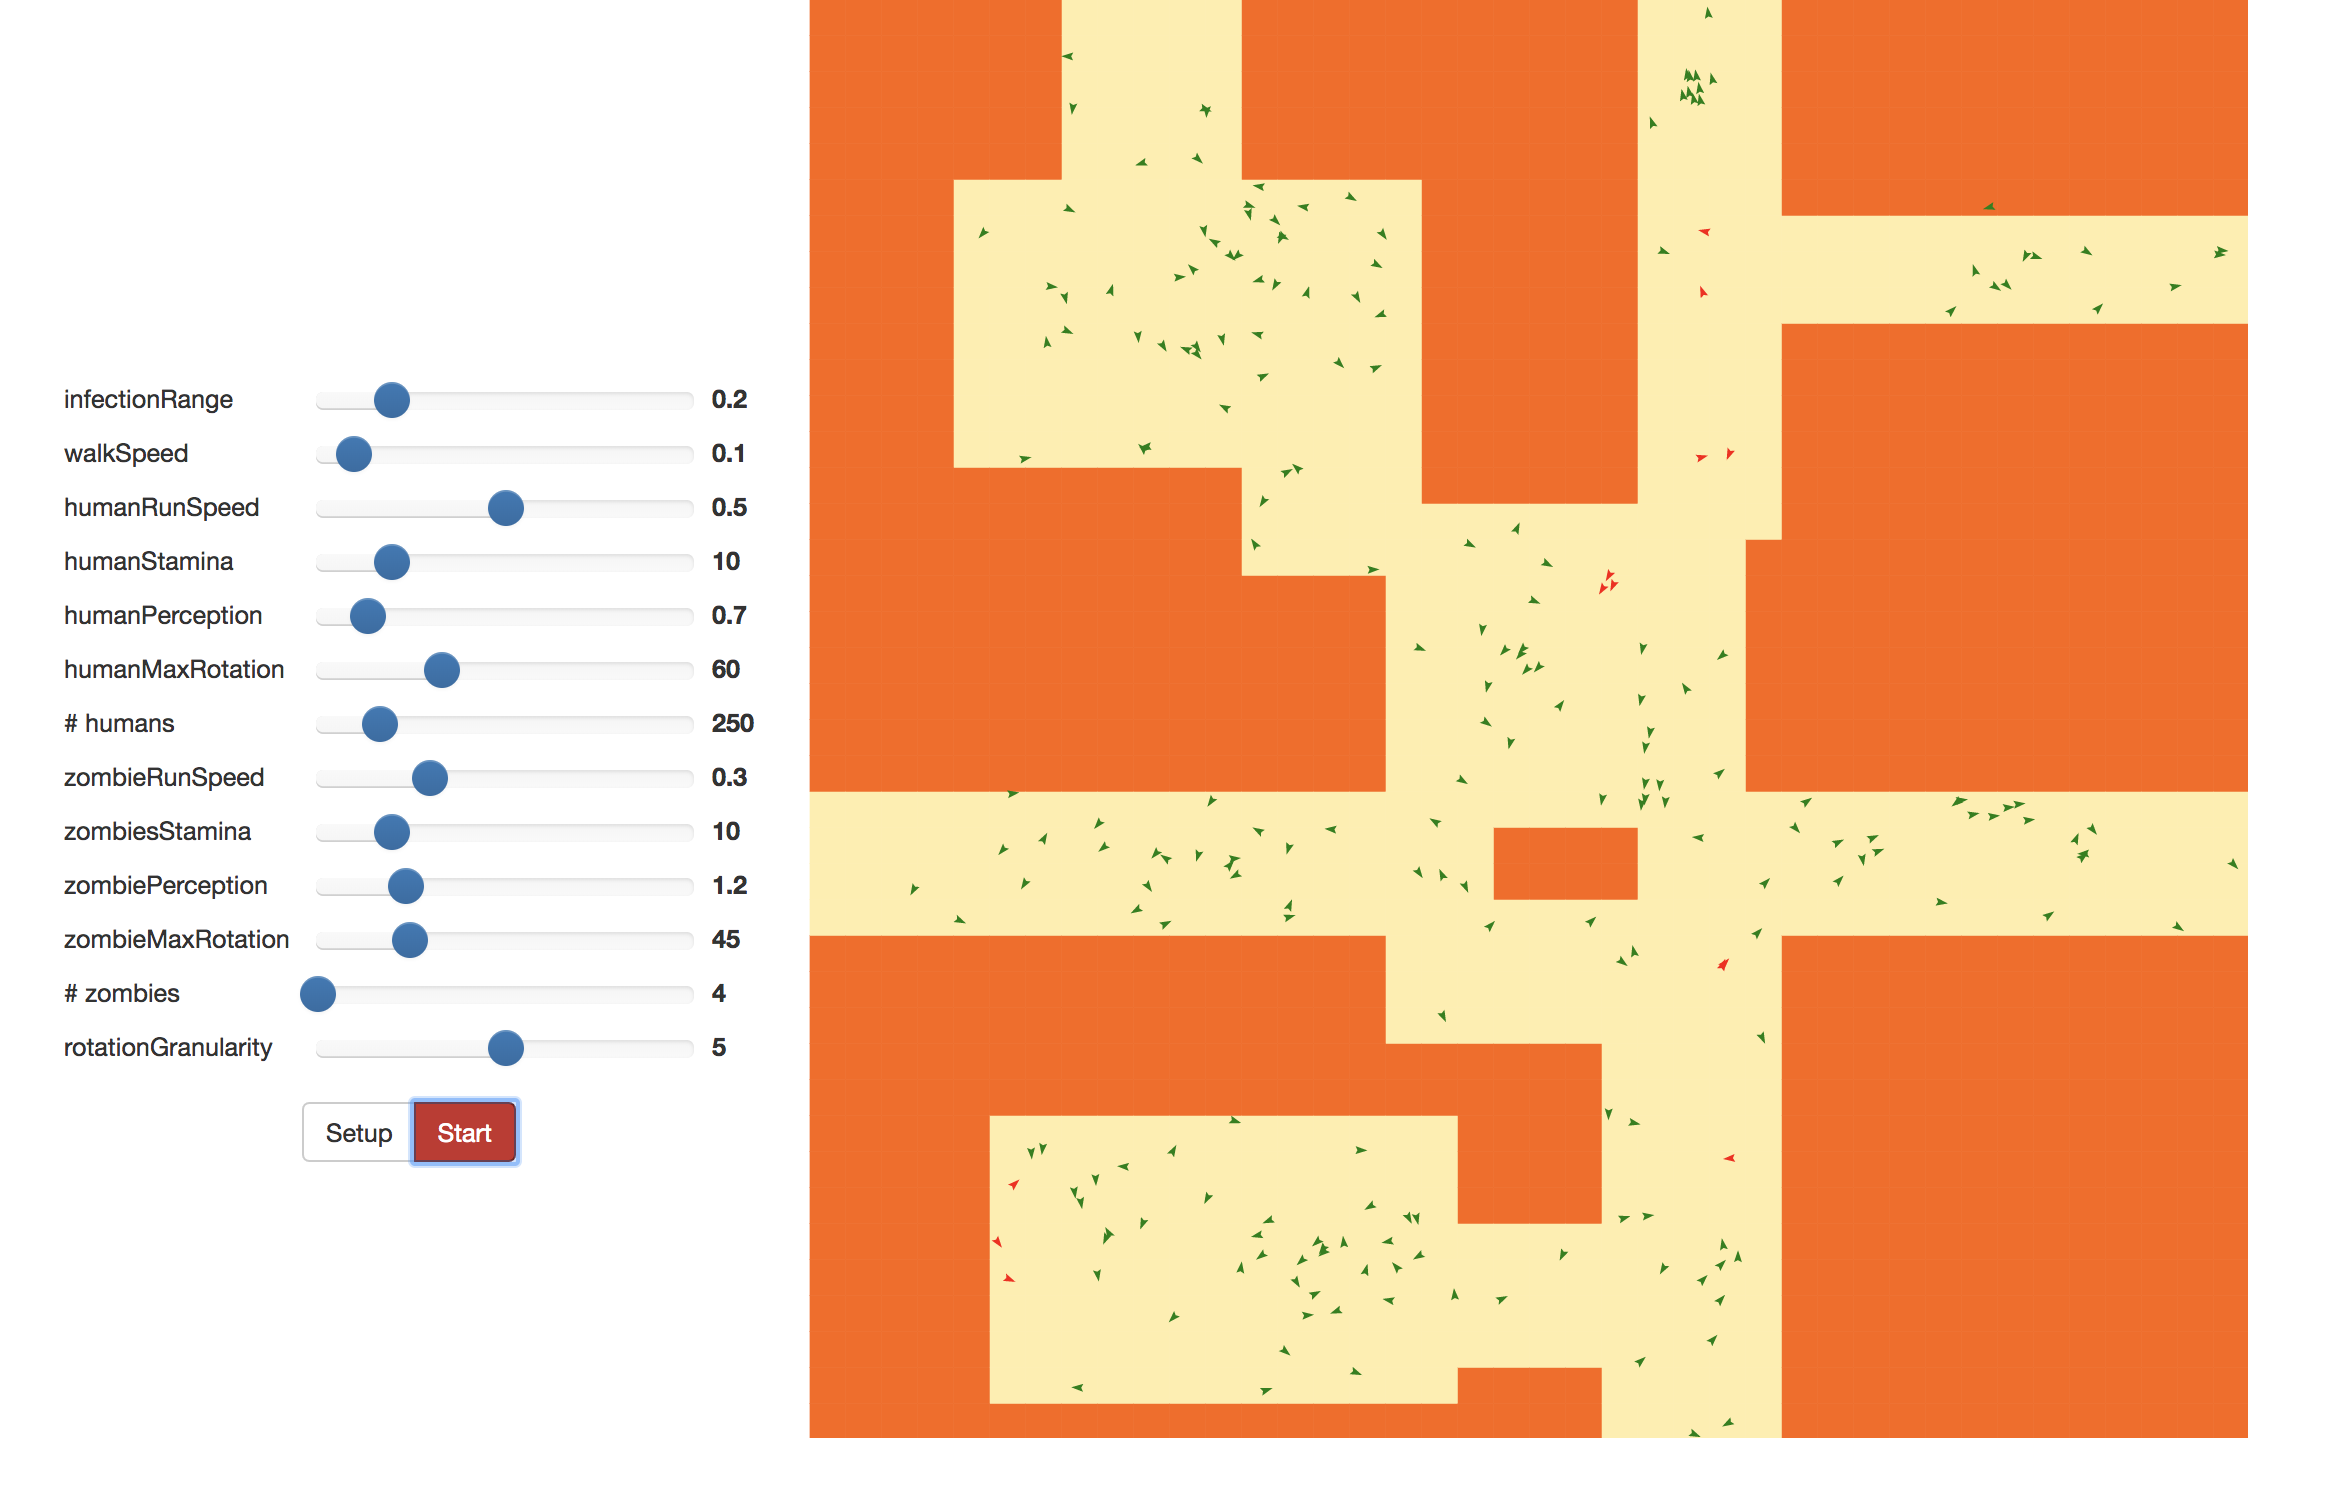
\includegraphics[width=\textwidth]{figures/zombieGUI.png}
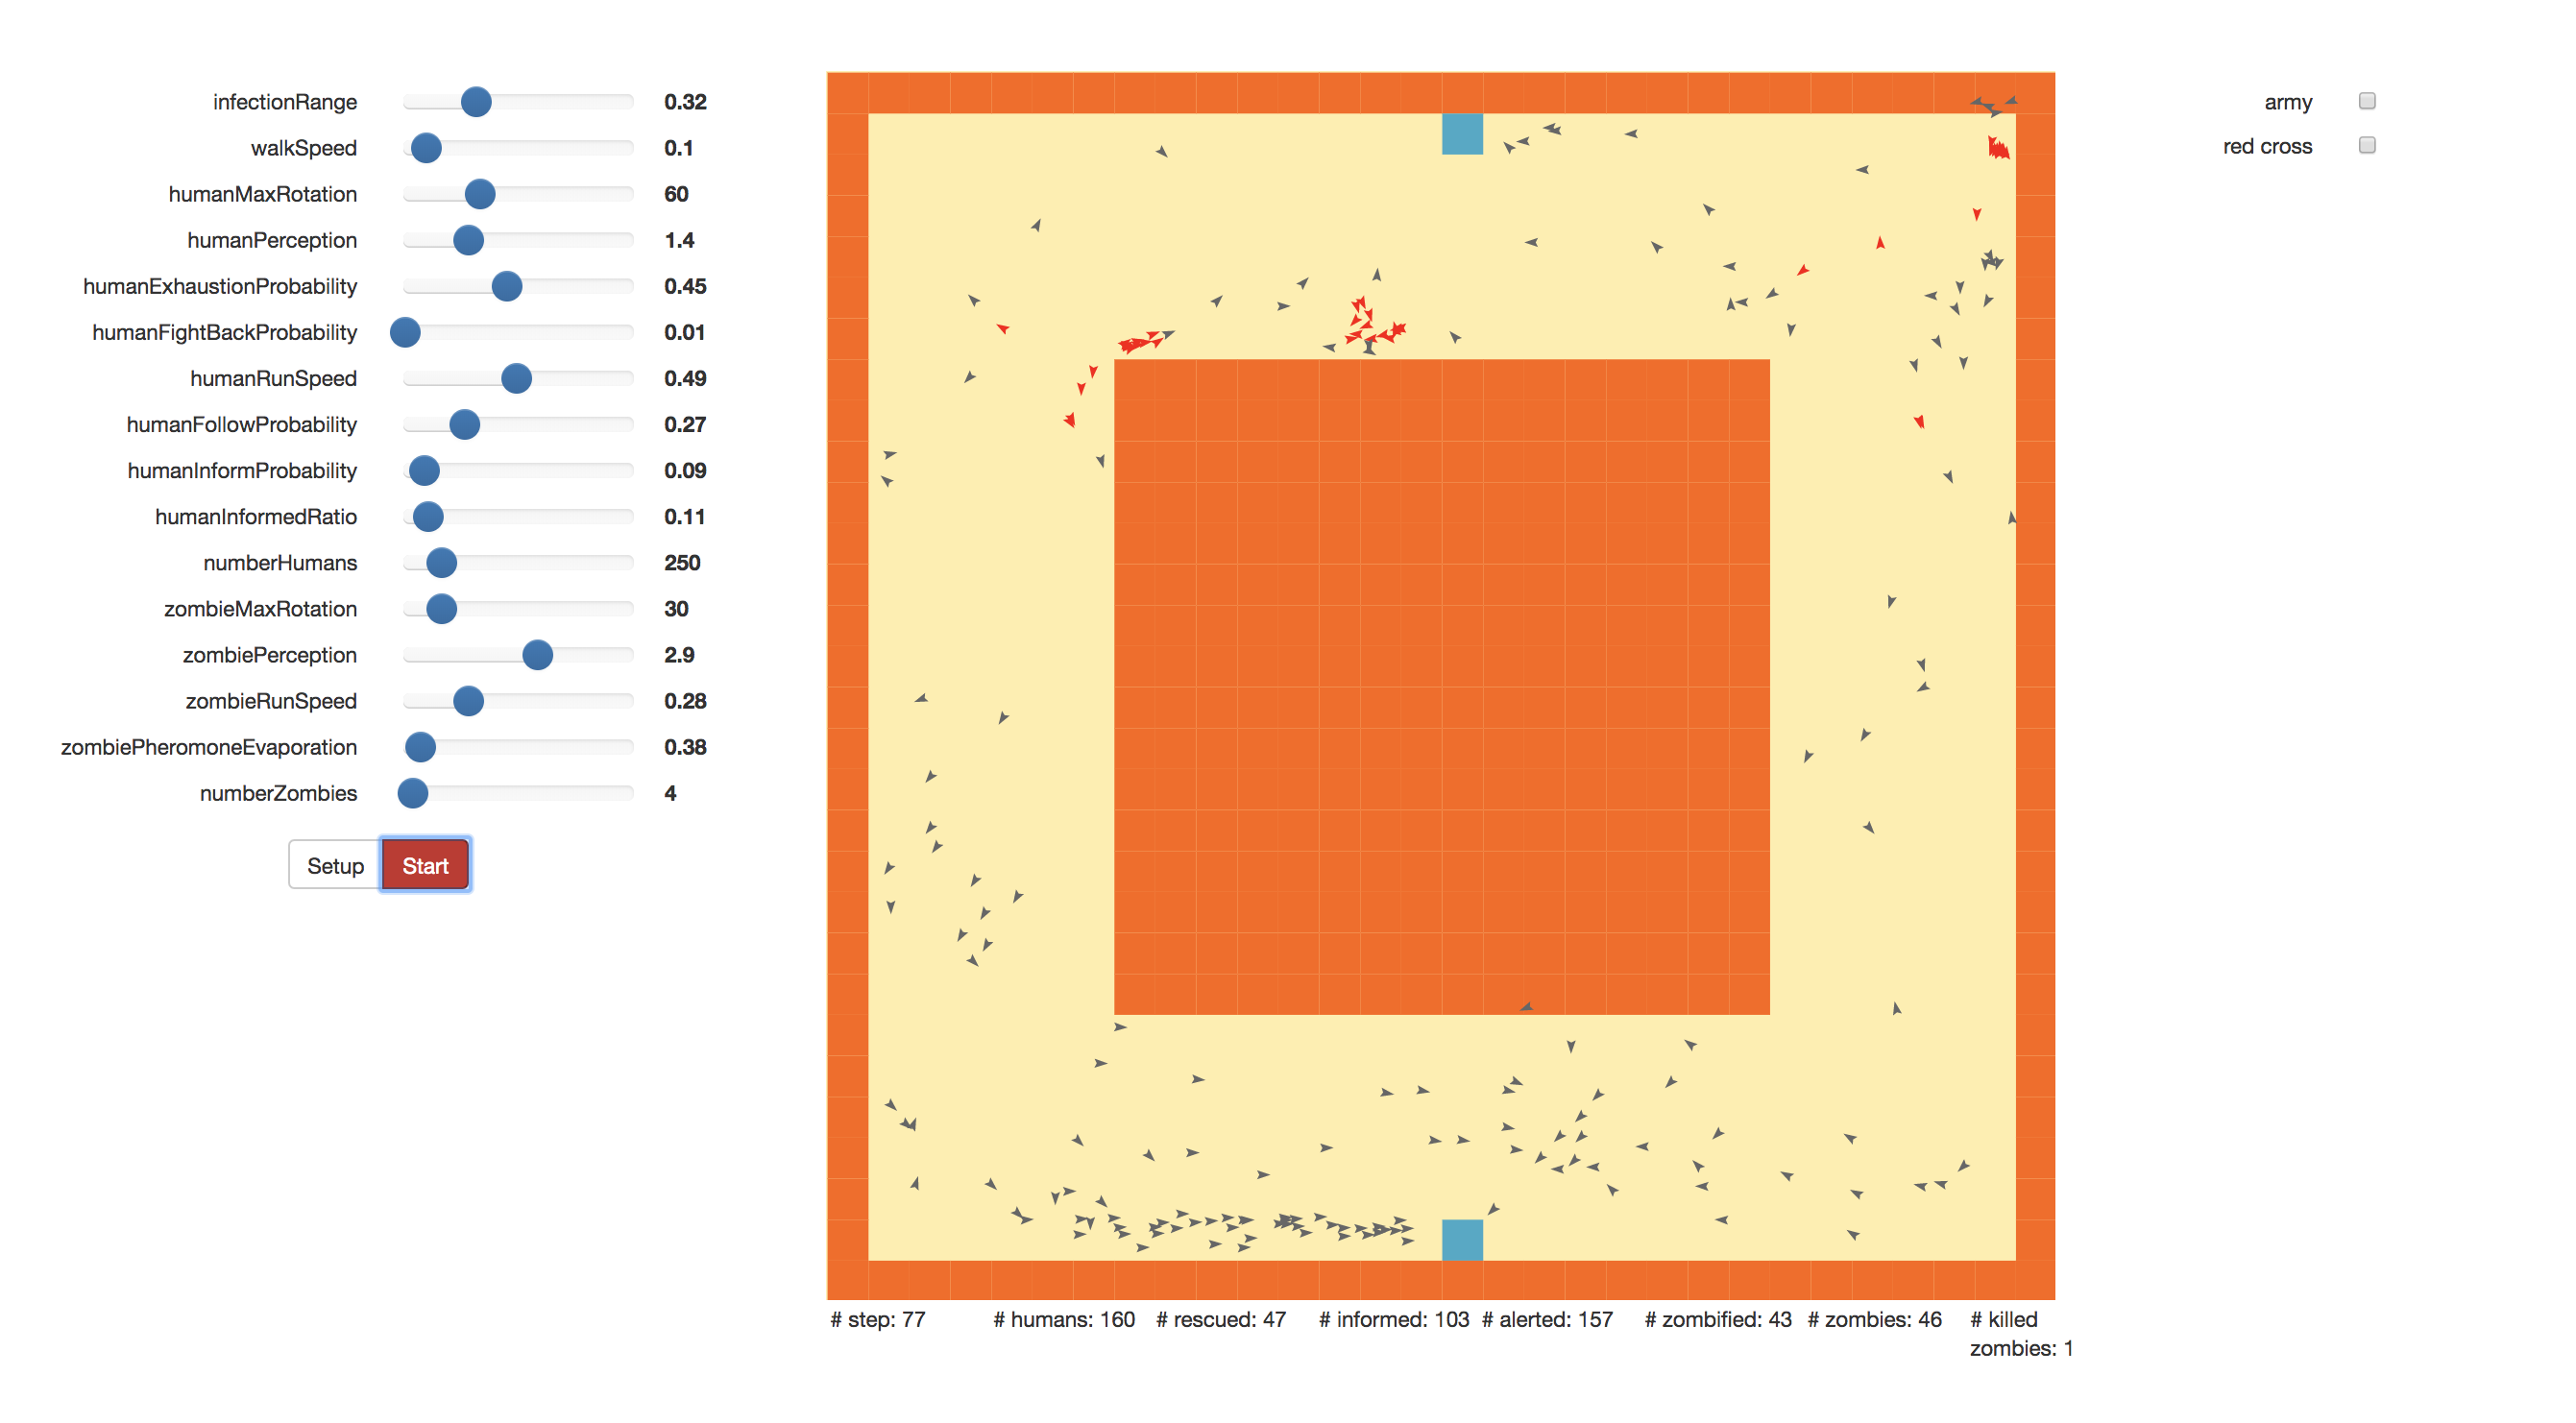
\includegraphics[width=\textwidth]{figures/zombieland_gui.png}
\end{center}

\medskip

\footnotesize

\textit{Local scale agent-based model}

}

\sframe{Let's get your hands on it}{
  
  \begin{itemize}
  	\item A submodel is available at  \url{https://om.exmodelo.org/coop}. Try the GUI and changing parameters
  	\item Most of next courses will be based on that model (additional processes will be detailed when needed)
  \end{itemize}
  
}



\sframe{Overview of the model}{

\begin{itemize}
	\item Simulate agent-level collective movements at the scale of a district
	\item Include behavioral processes for human (panic, search for rescues, \ldots) and zombies (self-organization, spontaneous attacks, \ldots), which can be adapted to local settings
	\item Include realistic pedestrian dynamics and realistic spatial configuration, which can be applied to local configuration
\end{itemize}

\medskip

\justify

\textbf{Objective of the model: } better understand the Zombie invasion process; possible applications to optimal policies and behavioral prevention to minimize the impact of recurring invasions

\medskip

\textbf{Issue with model application: } model has many parameters and processes, model behavior is unknown, application may be strongly case-dependent

\medskip

$\rightarrow$ \textit{we need \textbf{YOU} to understand this model to save the world}


}

\sframe{Basic processes and parameters}{

\begin{itemize}
	\item Humans and Zombies walk/run randomly (smoothed random walk) in an open urban space (movement parameters: rotation angle, walk and run speed)
	\item Interactions: human flee from zombie, zombies run for food, fight when encounter
	\item Humans can be rescued and information on the existence of rescues propagates between humans
	\item Additional processes in a multi-modeling approach (army, vaccination, \ldots)
\end{itemize}

}


\sframe{Pedestrian simulation}{

  % a bit of literature on pedestrian models

Multiple approaches to pedestrian simulations:

\medskip

\begin{itemize}
	\item Social force models \cite{helbing1995social}
	\item Granular flows \cite{cristiani2011multiscale}
	\item Behavioral models \cite{antonini2006discrete}
	\item Cellular automatons \cite{burstedde2001simulation}
	\item Potential field \cite{jian2014perceived}
\end{itemize}

\medskip

\textit{The ZOMBIE model takes the last approach, relatively realistic in a panic setting}

}


\sframe{Pedestrian potential field model}{

\begin{center}
	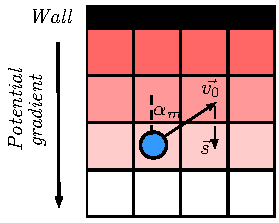
\includegraphics[height=0.8\textheight]{pedestrian}
\end{center}

\medskip



}


\sframe{Agents state machines}{

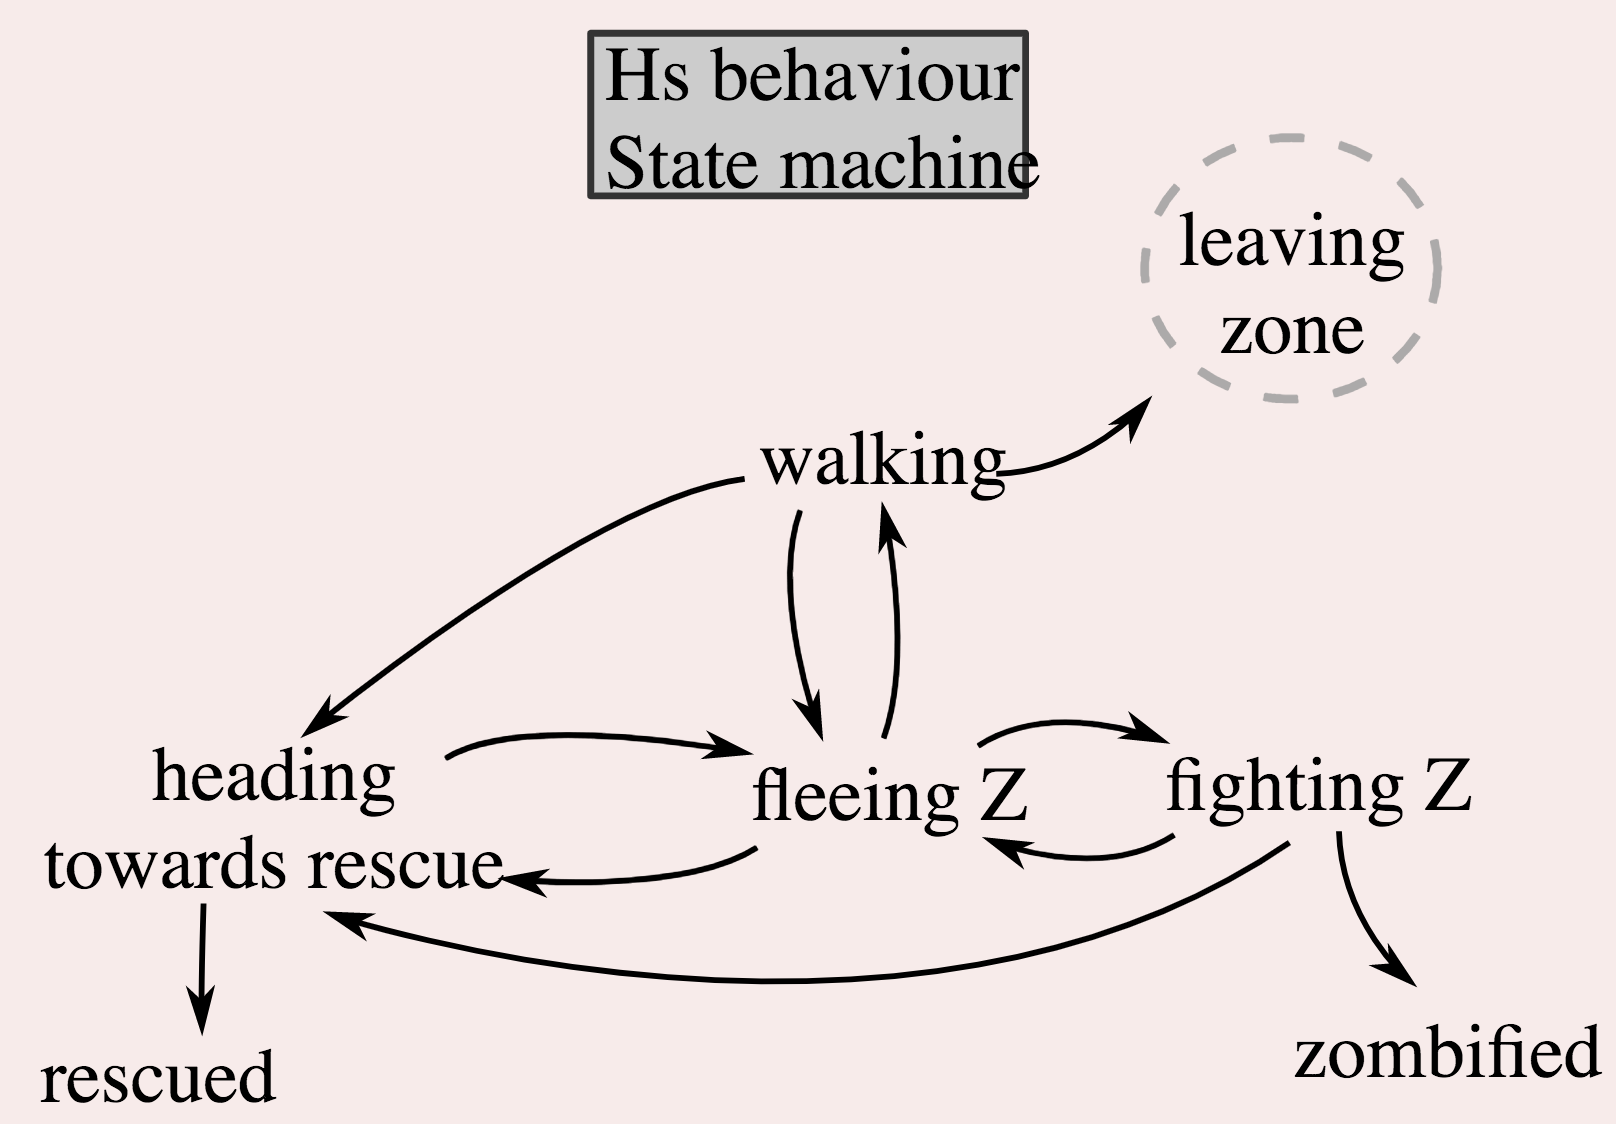
\includegraphics[width=0.51\textwidth]{figures/humanStateMachine.png}\hspace{0.2cm}
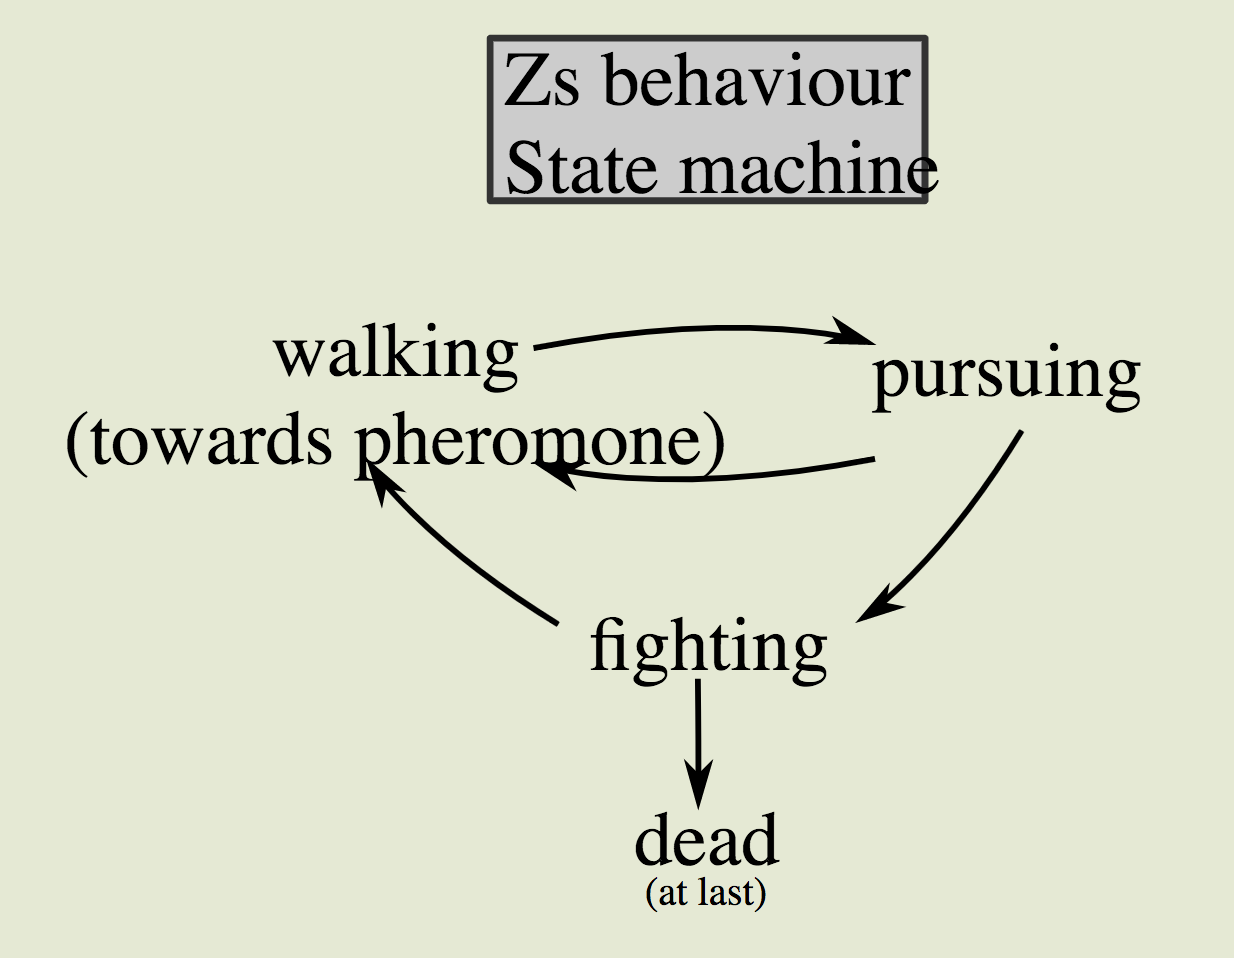
\includegraphics[width=0.46\textwidth]{figures/zombieStateMachine.png}

% launch simu https://om.exmodelo.org/coop/

}

\sframe{Information and rescues}{
 
 \begin{itemize}
 	\item Some spots allows informed humans to be rescued and get out of the world
 	\item An initial ratio of humans \texttt{humanInformRatio} is informed of the existence of rescues
 	\item Informed humans which are not in a panicking state follow a specific potential field leading to rescues
 	\item A human can inform an other one at the same location with a probability \texttt{humanInformProbability}
 \end{itemize}
 
\medskip

\justify

With the additional parameter \texttt{humanFollowProbability} (probability for a human to begin running and follow when they encounter an other running human), the submodel with three parameters is aimed at studying cooperation between humans.
 
}


\sframe{Changing the world}{

\begin{center}
	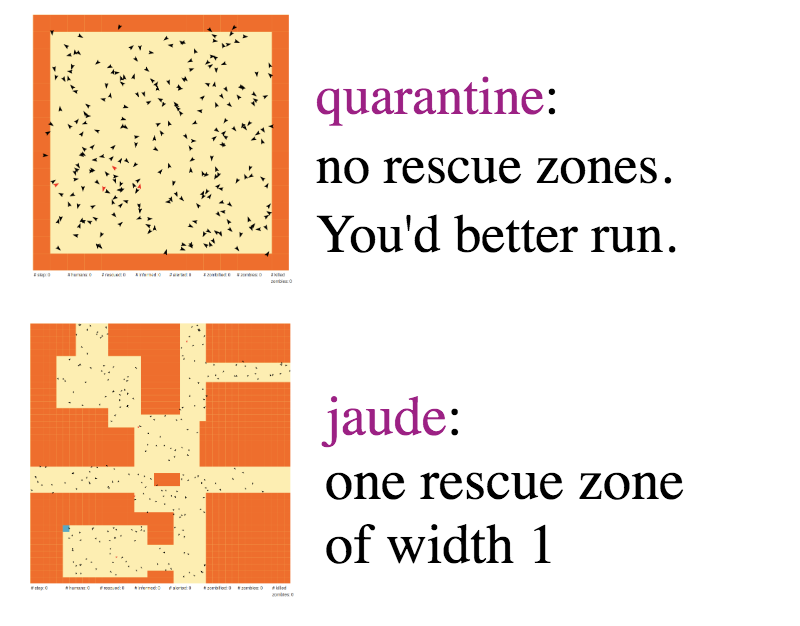
\includegraphics[height=0.6\textheight]{figures/worlds}	
\end{center}

\medskip

\textit{Alternative worlds \ldots and many more automatically generated (spatial sensitivity module on Wednesday)}


}


\sframe{A flexible and more general model}{

% one world on multi-modeling / deactivated parameters
% hidden parameters ?

% model as black box, pas besoin de connaitre exacetement tous les processus et parameteres

\begin{itemize}
	\item The general model, of which the three-parameter model is a particular case has more processes (deactivated or fixed)
	\item No need to know them for now, with the aim to understand the submodel on which we have the less knowledge
	\item Multi-modeling and model embedding (model as black box)
\end{itemize}

}


\sframe{The model in practice}{
 % scala impl + GUI -> layus on implementation / platform

 \begin{itemize}
 	\item Model implemented in scala (highly performant language mixing the best from functional programming and object programming)
 	\item Simple GUI for interactive exploration	
 	\item Integrated into OpenMOLE as a \texttt{jar} plugin in the GUI
 \end{itemize}


}




\sframe{The scala model}{

% main function zombieInvasion
% (transition for next course)

% say that plugin - as a jar

\textit{Scala syntax to run an execution of the model}

\bigskip
\bigskip

\centering

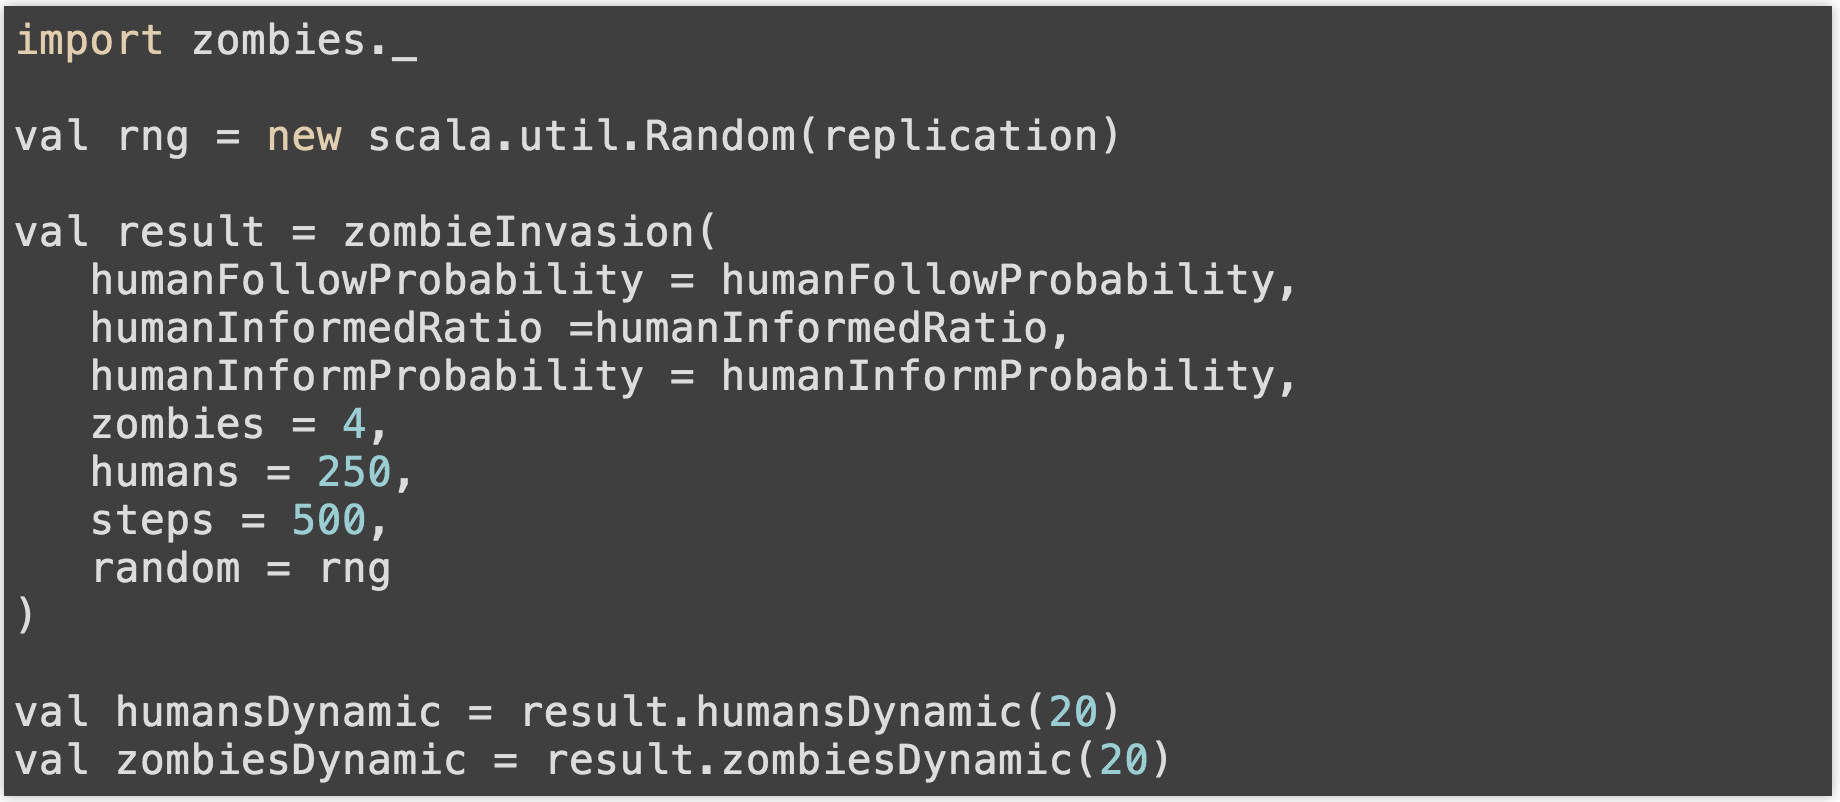
\includegraphics[width=\textwidth]{figures/zombies_scalaapi.png}

}


\backupbegin




%%%%%%%%%%%%%%%%%%%%%
\begin{frame}[allowframebreaks]
\frametitle{References}
\bibliographystyle{apalike}
\bibliography{biblio}
\end{frame}
%%%%%%%%%%%%%%%%%%%%%%%%%%%%


\backupend





\end{document}


